%
% $RCSfile: paper.tex,v $
%
% Copyright (c) 2004. Christian Heller. All rights reserved.
%
% No copying, altering, distribution or any other actions concerning this
% document, except after explicit permission by the author!
% At some later point in time, this document is planned to be put under
% the GNU FDL license. For now, _everything_ is _restricted_ by the author.
%
% http://www.cybop.net
% - Cybernetics Oriented Programming -
%
% http://www.resmedicinae.org
% - Information in Medicine -
%
% @author Christian Heller <christian.heller@tuxtax.de>
%

%
% The document class specifying the type of document.
%
\documentclass[a4paper,10pt]{llncs}

%
% The usepackages for document class.
%

% Paper format and font.
\usepackage{a4,times,helvet}

% Graphics.
\usepackage{graphicx}

%
% The space settings for edges (left, top, right, bottom).
%
\setlength{\hoffset}{-3,9cm}
\setlength{\voffset}{-3,6cm}
\setlength{\oddsidemargin}{4cm}
\setlength{\evensidemargin}{3cm}
\setlength{\topmargin}{1,5cm}
\setlength{\textwidth}{17cm}
\setlength{\textheight}{25cm}

%
% The hyphenation list.
%
%
% $RCSfile: hyphenation.tex,v $
%
% Copyright (c) 2002-2007. Christian Heller. All rights reserved.
%
% Permission is granted to copy, distribute and/or modify this document
% under the terms of the GNU Free Documentation License, Version 1.1 or
% any later version published by the Free Software Foundation; with no
% Invariant Sections, with no Front-Cover Texts and with no Back-Cover
% Texts. A copy of the license is included in the section entitled
% "GNU Free Documentation License".
%
% http://www.cybop.net
% - Cybernetics Oriented Programming -
%
% Version: $Revision: 1.2 $ $Date: 2007-08-01 13:59:00 $ $Author: christian $
% Authors: Christian Heller <christian.heller@tuxtax.de>
%

\hyphenation{abs-trac-tion}
\hyphenation{ac-tu-ally}
\hyphenation{ana-lyst}
\hyphenation{ana-ly-sis}
\hyphenation{an-cient}
\hyphenation{ap-pli-ca-tion}
\hyphenation{aris-to-tle}
\hyphenation{at-tri-bute}
\hyphenation{be-ing}
\hyphenation{ca-te-go-ri-za-tion}
\hyphenation{client}
\hyphenation{com-po-nen-ti-za-tion}
\hyphenation{com-pu-ter}
\hyphenation{con-fi-gure}
\hyphenation{con-nec-ted}
\hyphenation{cy-ber-ne-tics}
\hyphenation{cyboi}
\hyphenation{cybol}
\hyphenation{cybop}
\hyphenation{des-cribed}
\hyphenation{de-sign}
\hyphenation{de-ve-lop-ment}
\hyphenation{dis-crete}
\hyphenation{di-vide}
\hyphenation{do-main}
\hyphenation{dy-na-mic}
\hyphenation{eli-mi-nate}
\hyphenation{eli-mi-nates}
\hyphenation{eli-mi-na-tion}
\hyphenation{en-gi-nee-ring}
\hyphenation{en-vi-ron-ment}
\hyphenation{ex-pert}
\hyphenation{fi-gure}
\hyphenation{fle-xi-bi-li-sie-rung}
\hyphenation{fun-da-men-tal}
\hyphenation{hard-ware}
\hyphenation{hu-man}
\hyphenation{im-ple-men-ta-tion}
\hyphenation{in-he-rit}
\hyphenation{in-he-ri-tance}
\hyphenation{in-ter-pre-ter}
\hyphenation{java}
\hyphenation{know-ledge}
\hyphenation{lan-guage}
\hyphenation{li-ving}
\hyphenation{lo-gi-cal}
\hyphenation{ma-na-ge-ment}
\hyphenation{mea-ning-ful}
\hyphenation{me-cha-nism}
\hyphenation{me-mo-ry}
\hyphenation{me-thod}
\hyphenation{me-thods}
\hyphenation{mo-del-ling}
\hyphenation{na-ture}
\hyphenation{net-work}
\hyphenation{neu-ral}
\hyphenation{neu-ron}
\hyphenation{ne-ver-en-ding-ly}
\hyphenation{open}
\hyphenation{operating}
\hyphenation{ori-en-ted}
\hyphenation{over-come}
\hyphenation{par-ti-cu-lar}
\hyphenation{prin-ci-ple}
\hyphenation{pro-ba-bi-lis-tic}
\hyphenation{pro-ble-ma-tic}
\hyphenation{pro-gram-ming}
\hyphenation{res-pon-sible}
\hyphenation{re-u-sa-bi-li-ty}
\hyphenation{sci-ence}
\hyphenation{server}
\hyphenation{si-mi-lar}
\hyphenation{soft-ware}
\hyphenation{source}
\hyphenation{spe-cia-li-za-tion}
\hyphenation{spe-ci-fied}
\hyphenation{sta-tic}
\hyphenation{sta-ti-cally}
\hyphenation{sto-chas-tic}
\hyphenation{stone-on-stone}
\hyphenation{struc-ture}
\hyphenation{strug-gling}
\hyphenation{subs-ti-tu-ting}
\hyphenation{su-per-flu-ous}
\hyphenation{sup-ply-ing}
\hyphenation{sys-tem}
\hyphenation{taeu-schungs-ver-such}
\hyphenation{temp-lates}
\hyphenation{tes-ting}
\hyphenation{thin-king}
\hyphenation{un-en-li-vened}
\hyphenation{un-sa-tis-fy-ing}
\hyphenation{va-ry-ing}
\hyphenation{weigh-ted}
\hyphenation{zu-kunfts-si-che-re}


%
% This document is a scientific paper to be handed in for a conference.
%
% @version $Revision: 1.1 $ $Date: 2005-03-14 21:46:26 $ $Author: christian $
% @author Christian Heller <christian.heller@tuxtax.de>
% @author Christian Heller <christian.heller@tu-ilmenau.de>
%
\begin{document}
    \twocolumn
    \title{Flexible Software Architectures for Presentation Layers demonstrated on Medical Documentation with Episodes and Inclusion of Topological Report}
\author{Jens Bohl \(<\)info@jens-bohl.de\(>\)\\
Torsten Kunze \(<\)zone3@gmx.de\(>\)\\
Christian Heller \(<\)christian.heller@tu-ilmenau.de\(>\)\\
Ilka Philippow \(<\)ilka.philippow@tu-ilmenau.de\(>\)}
\institute{
Technical University of Ilmenau\\
Faculty for Computer Science and Automation\\
Institute for Theoretical and Technical Informatics\\
PF 100565, Max-Planck-Ring 14, 98693 Ilmenau, Germany\\
http://www.tu-ilmenau.de, fon: +49-(0)3677-69-1230, fax: +49-(0)3677-69-1220}
\maketitle

    \maketitle
    %
% $RCSfile: abstract.tex,v $
%
% Copyright (c) 2001-2004. Christian Heller. All rights reserved.
%
% No copying, altering, distribution or any other actions concerning this
% document, except after explicit permission by the author!
% At some later point in time, this document is planned to be put under
% the GNU FDL license. For now, _everything_ is _restricted_ by the author.
%
% http://www.cybop.net
% - Cybernetics Oriented Programming -
%
% http://www.resmedicinae.org
% - Information in Medicine -
%
% @author Christian Heller <christian.heller@tuxtax.de>
%

\begin{abstract}
This article reports about an ongoing research investigating the possibilities
for applying inter-disciplinary concepts to software system design. The new
resulting programming philosophy is based on firstly, a distinction of statics
and dynamics, secondly a knowledge schema structuring models and their meta
information hierarchically, and thirdly the separation of state- and logic
knowledge. It solves many of the problems existing in classical programming
paradigms and languages and may have the potential to replace these in the long
run.\\
\textbf{Keywords:} Knowledge Abstraction, Cybernetics Oriented Programming,
CYBOP, Software Design
\end{abstract}

    %
% $RCSfile: introduction.tex,v $
%
% Copyright (c) 2002-2007. Christian Heller. All rights reserved.
%
% Permission is granted to copy, distribute and/or modify this document
% under the terms of the GNU Free Documentation License, Version 1.1 or
% any later version published by the Free Software Foundation; with no
% Invariant Sections, with no Front-Cover Texts and with no Back-Cover
% Texts. A copy of the license is included in the section entitled
% "GNU Free Documentation License".
%
% http://www.cybop.net
% - Cybernetics Oriented Programming -
%
% Version: $Revision: 1.1 $ $Date: 2007-07-17 20:02:36 $ $Author: christian $
% Authors: Christian Heller <christian.heller@tuxtax.de>
%

\chapter{Introduction}
\label{introduction_heading}
\index{Introduction}

This is just a test \cite{zimmermann} citation.

%
% $RCSfile: terminology.tex,v $
%
% Copyright (C) 2002-2008. Christian Heller.
%
% Permission is granted to copy, distribute and/or modify this document
% under the terms of the GNU Free Documentation License, Version 1.1 or
% any later version published by the Free Software Foundation; with no
% Invariant Sections, with no Front-Cover Texts and with no Back-Cover
% Texts. A copy of the license is included in the section entitled
% "GNU Free Documentation License".
%
% http://www.cybop.net
% - Cybernetics Oriented Programming -
%
% http://www.resmedicinae.org
% - Information in Medicine -
%
% Version: $Revision: 1.1 $ $Date: 2008-08-19 20:41:09 $ $Author: christian $
% Authors: Christian Heller <christian.heller@tuxtax.de>
%

\subsection{Terminology}
\label{terminology_heading}
\index{Terminology}
\index{Lexicon}
\index{Vocabulary}
\index{Nomenclature}
\index{Hierarchy}
\index{Semantic Link}
\index{Directed Acyclic Graph}
\index{DAG}

While a \emph{Lexicon} is a list of pure words, a \emph{Terminology} (sometimes
called \emph{Vocabulary}) can also contain phrases. Because it is a fixed list
of lots of terms, a terminology should exclude any link to a separate list of
concepts. When a terminology contains additional instructions describing how to
interpret each term, or dictating when to choose one over another
(prioritisation), it may be called a \emph{Nomenclature}. The knowledge schema
proposed in this work (chapter \ref{knowledge_schema_heading}) shall be capable
of storing codes of various terminology systems.

Lexicon and terminology stand for a \emph{Set} of words or terms, respectively.
To bring some structure into such a set, terms or concepts need to be ordered,
that is organised through a system of links, into a \emph{Hierarchy}, which
Rogers \cite{rogers} defines as a:

\begin{quote}
    \ldots\ tree-like structure, where things at the top of the tree are in some
    way more general or abstract than the things lower down. The nature of each
    link between each level in the tree may be explicit or only implied, and
    more than one flavour of semantic link can be used to build the tree (in
    which case it may be called a \emph{Mixed Hierarchy}).
\end{quote}

Kinds of hierarchies, as means of organisation, are:

\begin{itemize}
    \item[-] \emph{Subsumption Hierarchy} (Classification, Taxonomy): only
        \emph{is-a} relationships exist between parent-child pairs in the tree
    \item[-] \emph{Uniaxial Hierarchy:} each concept only ever has one parent,
        though it can have more than one child
    \item[-] \emph{Multiaxial Hierachy:} each concept can have more than one
        parent as well as more than one child
    \item[-] \emph{Exhaustive Multiaxial Hierarchy:} all concepts have all the
        parents as well as all the children they should have
\end{itemize}

As organisation \emph{Rules} count:

\begin{itemize}
    \item[-] \emph{Formalism}: an explicitly expressed set of rules, like the
        specification for how to tell what should (not) be a parent of a concept
    \item[-] \emph{Concept System} (Model): a system of \emph{Symbols} that
        stand in for concepts and/ or the links between them, and which may or
        may not be intended to be processed with reference to some formalism
    \item[-] \emph{Partonomy} (Mereology): a system of concepts and links
        intended to represent whole-part relationships specifically
\end{itemize}

On a yet higher abstract level, a \emph{Data Structure} may hold organisations
of concepts. Various types of data structures are:

\begin{itemize}
    \item[-] \emph{Network}: a mesh-like structure that connects terms or concepts
        using links; a hierarchy can be thought of as simple case of a network
    \item[-] \emph{Graph}: a network
    \item[-] \emph{Directed Graph}: a network in which each link has a \emph{Direction}
    \item[-] \emph{Directed Acyclic Graph} (DAG): a directed graph free of loops
\end{itemize}

A knowledge template expressed in the language that will be defined in chapter
\ref{cybernetics_oriented_language_heading} describes an uniaxial hierarchy,
that is its sub concepts have just one parent node. Its structure follows the
partonomy (mereology) organisation rules and represents a DAG.

%
% $RCSfile: cybernetics_oriented_programming.tex,v $
%
% Copyright (c) 2002-2007. Christian Heller. All rights reserved.
%
% Permission is granted to copy, distribute and/or modify this document
% under the terms of the GNU Free Documentation License, Version 1.1 or
% any later version published by the Free Software Foundation; with no
% Invariant Sections, with no Front-Cover Texts and with no Back-Cover
% Texts. A copy of the license is included in the section entitled
% "GNU Free Documentation License".
%
% http://www.cybop.net
% - Cybernetics Oriented Programming -
%
% Version: $Revision: 1.1 $ $Date: 2007-07-17 20:02:36 $ $Author: christian $
% Authors: Christian Heller <christian.heller@tuxtax.de>
%

\section{Cybernetics Oriented Programming}
\label{cybernetics_oriented_programming_heading}
\index{Cybernetics Oriented Programming}

The \emph{Cybernetics Oriented Programming} (CYBOP) software development theory
suggests to ...

%
% $RCSfile: software_engineering_process.tex,v $
%
% Copyright (c) 2002-2007. Christian Heller. All rights reserved.
%
% Permission is granted to copy, distribute and/or modify this document
% under the terms of the GNU Free Documentation License, Version 1.1 or
% any later version published by the Free Software Foundation; with no
% Invariant Sections, with no Front-Cover Texts and with no Back-Cover
% Texts. A copy of the license is included in the section entitled
% "GNU Free Documentation License".
%
% http://www.cybop.net
% - Cybernetics Oriented Programming -
%
% Version: $Revision: 1.1 $ $Date: 2007-07-17 20:02:36 $ $Author: christian $
% Authors: Christian Heller <christian.heller@tuxtax.de>
%

\subsection{Software Engineering Process}
\label{software_engineering_process_heading}
\index{Software Engineering Process}

Although hundreds of variations, with or without iterations, exist, a standard
\emph{Software Engineering Process} (SEP) consists of the phases: \emph{Analysis},
\emph{Design} and \emph{Implementation}, as illustrated in figure
\ref{software_engineering_process_figure}.

\begin{figure}[ht]
    \begin{center}
        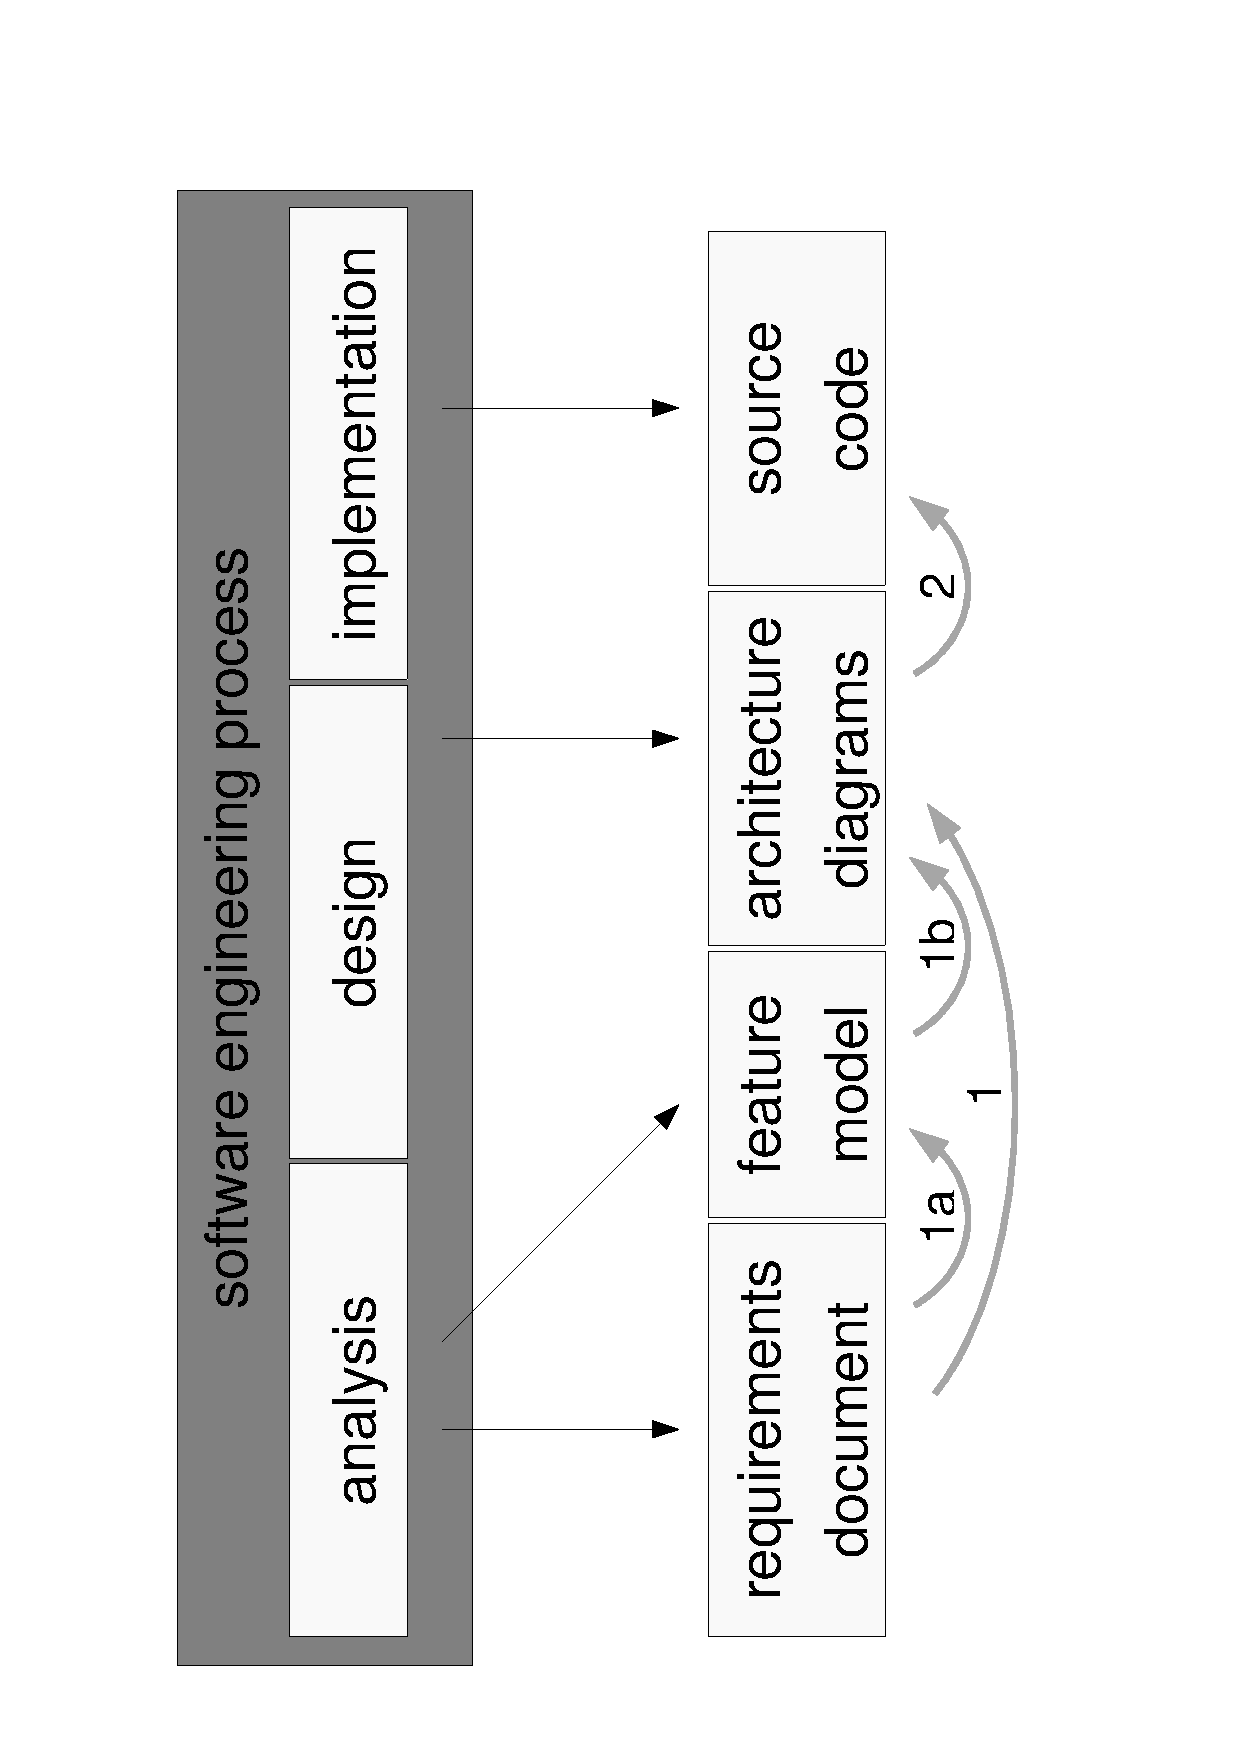
\includegraphics[scale=0.3,angle=-90]{graphics/gaps.pdf}
        \caption{Standard Software Engineering Process}
        \label{software_engineering_process_figure}
    \end{center}
\end{figure}

%
% $RCSfile: interpretation.tex,v $
%
% Copyright (c) 2002-2007. Christian Heller. All rights reserved.
%
% Permission is granted to copy, distribute and/or modify this document
% under the terms of the GNU Free Documentation License, Version 1.1 or
% any later version published by the Free Software Foundation; with no
% Invariant Sections, with no Front-Cover Texts and with no Back-Cover
% Texts. A copy of the license is included in the section entitled
% "GNU Free Documentation License".
%
% http://www.cybop.net
% - Cybernetics Oriented Programming -
%
% Version: $Revision: 1.1 $ $Date: 2007-07-17 20:02:36 $ $Author: christian $
% Authors: Christian Heller <christian.heller@tuxtax.de>
%

\subsection{Interpretation}
\label{inerpretation_heading}
\index{Interpretation}

CYBOP
CYBOL
CYBOI

\begin{figure}[ht]
    \begin{center}
        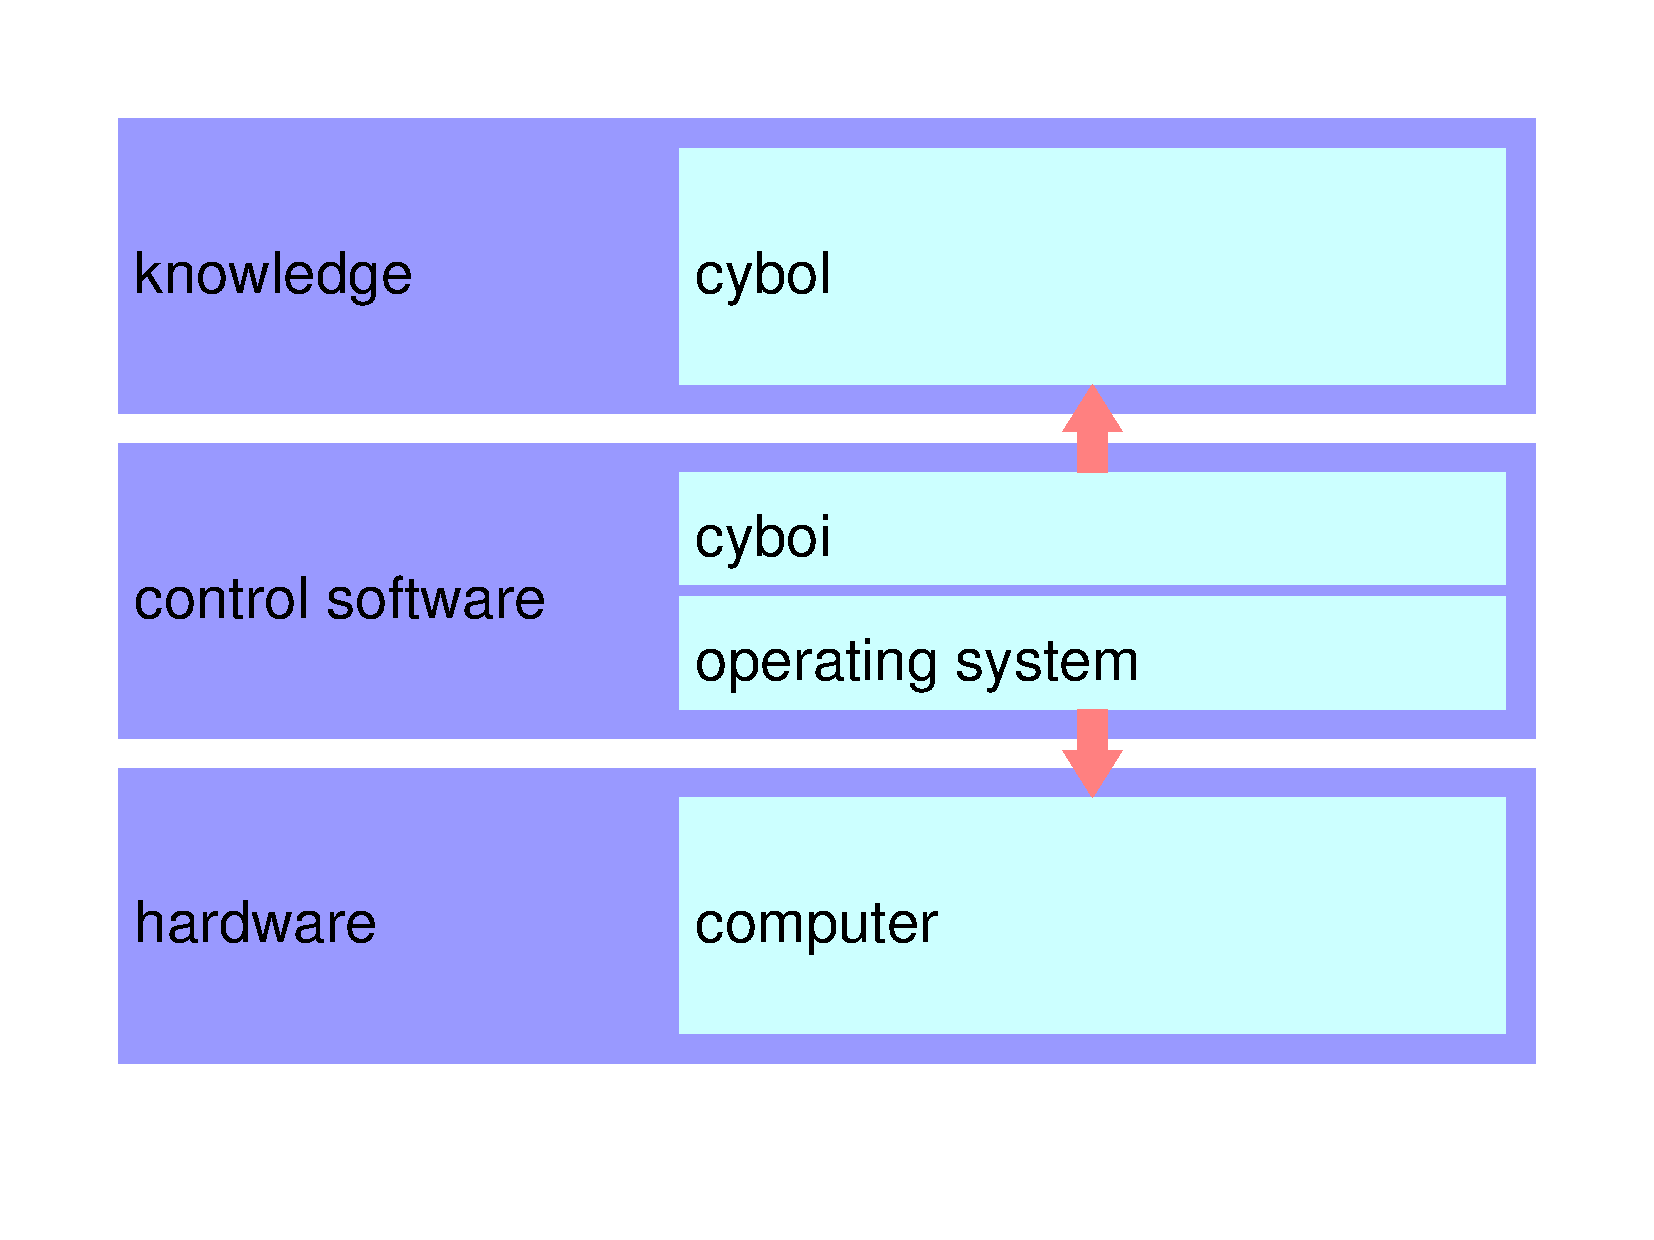
\includegraphics[scale=0.3,angle=-90]{graphics/connection.pdf}
        \caption{CYBOL Interpretation}
        \label{cybol_interpretation_figure}
    \end{center}
\end{figure}


%
% $RCSfile: extensible_markup_language.tex,v $
%
% Copyright (c) 2002-2007. Christian Heller. All rights reserved.
%
% Permission is granted to copy, distribute and/or modify this document
% under the terms of the GNU Free Documentation License, Version 1.1 or
% any later version published by the Free Software Foundation; with no
% Invariant Sections, with no Front-Cover Texts and with no Back-Cover
% Texts. A copy of the license is included in the section entitled
% "GNU Free Documentation License".
%
% http://www.cybop.net
% - Cybernetics Oriented Programming -
%
% Version: $Revision: 1.1 $ $Date: 2007-07-17 20:02:36 $ $Author: christian $
% Authors: Christian Heller <christian.heller@tuxtax.de>
%

\section{Extensible Markup Language}
\label{extensible_markup_language_heading}
\index{Extensible Markup Language}

The \emph{Extensible Markup Language} (XML) is ...


    %
% $RCSfile: pattern.tex,v $
%
% Copyright (c) 2004. Christian Heller. All rights reserved.
%
% No copying, altering, distribution or any other actions concerning this
% document, except after explicit permission by the author!
% At some later point in time, this document is planned to be put under
% the GNU FDL license. For now, _everything_ is _restricted_ by the author.
%
% http://www.cybop.net
% - Cybernetics Oriented Programming -
%
% http://www.resmedicinae.org
% - Information in Medicine -
%
% @author Christian Heller <christian.heller@tuxtax.de>
%

\section{Pattern}
\label{pattern_heading}

%
% $RCSfile: definition.tex,v $
%
% Copyright (c) 2004. Christian Heller. All rights reserved.
%
% No copying, altering, distribution or any other actions concerning this
% document, except after explicit permission by the author!
% At some later point in time, this document is planned to be put under
% the GNU FDL license. For now, _everything_ is _restricted_ by the author.
%
% http://www.cybop.net
% - Cybernetics Oriented Programming -
%
% http://www.resmedicinae.org
% - Information in Medicine -
%
% @author Christian Heller <christian.heller@tuxtax.de>
%

\subsection{Definition}
\label{definition_heading}

\emph{Patterns}, in a more correct form called \emph{Software Patterns}, represent
solutions for recurring software design problems and can be understood as
recommendations for how to build software in an elegant way. In the past, more
detailed definitions have been given by meanwhile well-known authors.

Christopher Alexander, an architect and urban planner, writes \cite{alexander}:
\textit{Each pattern describes a problem which occurs over and over again in
our environment, and then describes the core of the solution to that problem,
in such a way that you can use this solution a million times over, without ever
doing it the same way twice.} He gave this definition primarily for problems
occuring in architecture, construction, and urban/regional planning, but it can
be applied in the same manner to software design, as done first by Ward
Cunningham and others \cite{portland}.

The systems designer Swift \cite{designmatrix} sees a pattern as:
\textit{essentially a morphological law, a relationship among parts (pattern
components) within a particular context. Specifically, a pattern expresses a
relationship among parts that resolves problems that would exist if the
relationship were missing. As patterns express these relationships, they are
not formulae or algorithms, but rather loose rules of thumb or heuristics.}

The \emph{Gang of Four} (Erich Gamma et al.) applied Alexander's definition to
object oriented software and created a whole catalogue of design patterns
\cite{gamma1995}. After them, patterns are: \textit{Structured models of
thinking that represent reusable solutions for one-and-the-same design problem.
They shall support the development, maintenance and extension of large software
systems, while being independent from concrete implementation languages.} The
experts identified four basic elements of each pattern: \emph{Name},
\emph{Problem}, \emph{Solution} and \emph{Consequences} (advantages and
disadvantages).

For Frank Buschmann et al., software patterns contain the knowledge of
experienced software engineers and help to improve the quality of decision
making \cite{buschmann}. In his opinion, they are \emph{Problem Solution Pairs},
that is basic solutions for problems that already occured in a similar way before.

Martin Fowler means that: \textit{A pattern is some idea that already was
helpful in a practical context and will probably be useful in other contexts,
too.} \cite{fowler1997}. After him, patterns, however they are written, have
four essential parts: \emph{Context}, \emph{Problem}, \emph{Forces} and
\emph{Solution}.

Depending on their experience, software developers produce good or bad solutions.
One possibility to improve less well-done designs or to extend legacy systems
are \emph{Anti-Patterns} (telling how to go from a problem to a bad design),
or the contrasting \emph{Amelioration Patterns} (telling how to go from a bad-
to a good solution) \cite{portland}. Both help finding patterns in wrong-designed
systems, to improve these.

There are efforts to combine patterns to form a \emph{Pattern Language}, also
called \emph{Pattern System} \cite{buschmann}. Such systems describe
dependencies between patterns, specify rules for pattern combination and show
how patterns can be implemented and used in software development practice.

%
% $RCSfile: classification.tex,v $
%
% Copyright (C) 2002-2008. Christian Heller.
%
% Permission is granted to copy, distribute and/or modify this document
% under the terms of the GNU Free Documentation License, Version 1.1 or
% any later version published by the Free Software Foundation; with no
% Invariant Sections, with no Front-Cover Texts and with no Back-Cover
% Texts. A copy of the license is included in the section entitled
% "GNU Free Documentation License".
%
% http://www.cybop.net
% - Cybernetics Oriented Programming -
%
% http://www.resmedicinae.org
% - Information in Medicine -
%
% Version: $Revision: 1.1 $ $Date: 2008-08-19 20:41:05 $ $Author: christian $
% Authors: Christian Heller <christian.heller@tuxtax.de>
%

\subsubsection{Classification}
\label{classification_heading}
\index{Classification}
\index{Class}
\index{Attribute}
\index{Method}
\index{Structured Data Type}
\index{Struct}
\index{Record}
\index{Structured and Procedural Programming}
\index{SPP}
\index{Java}
\index{Global Variable}
\index{Instance}
\index{Object}
\index{Instantiation}
\index{Abstract Class}
\index{Interface}
\index{Inner Class}
\index{Bundling of Attributes and Methods}

The main idea of object oriented programming is to structure program code into
\emph{Classes} owning \emph{Attributes} and \emph{Methods} (figure
\ref{classification_figure}). They are comparable to the structured data types
(\emph{struct}, \emph{record}) of \emph{Structured and Procedural Programming}
(SPP) (section \ref{structured_and_procedural_programming_heading}) that can
own fields representing properties, but not behaviour. A class definition in
\emph{Java} source code looks like this:

\begin{scriptsize}
    \begin{verbatim}
    public class Example {
        private Type attribute;
        public void method(Type parameter) {
        }
    }
    \end{verbatim}
\end{scriptsize}

\begin{figure}[ht]
    \begin{center}
        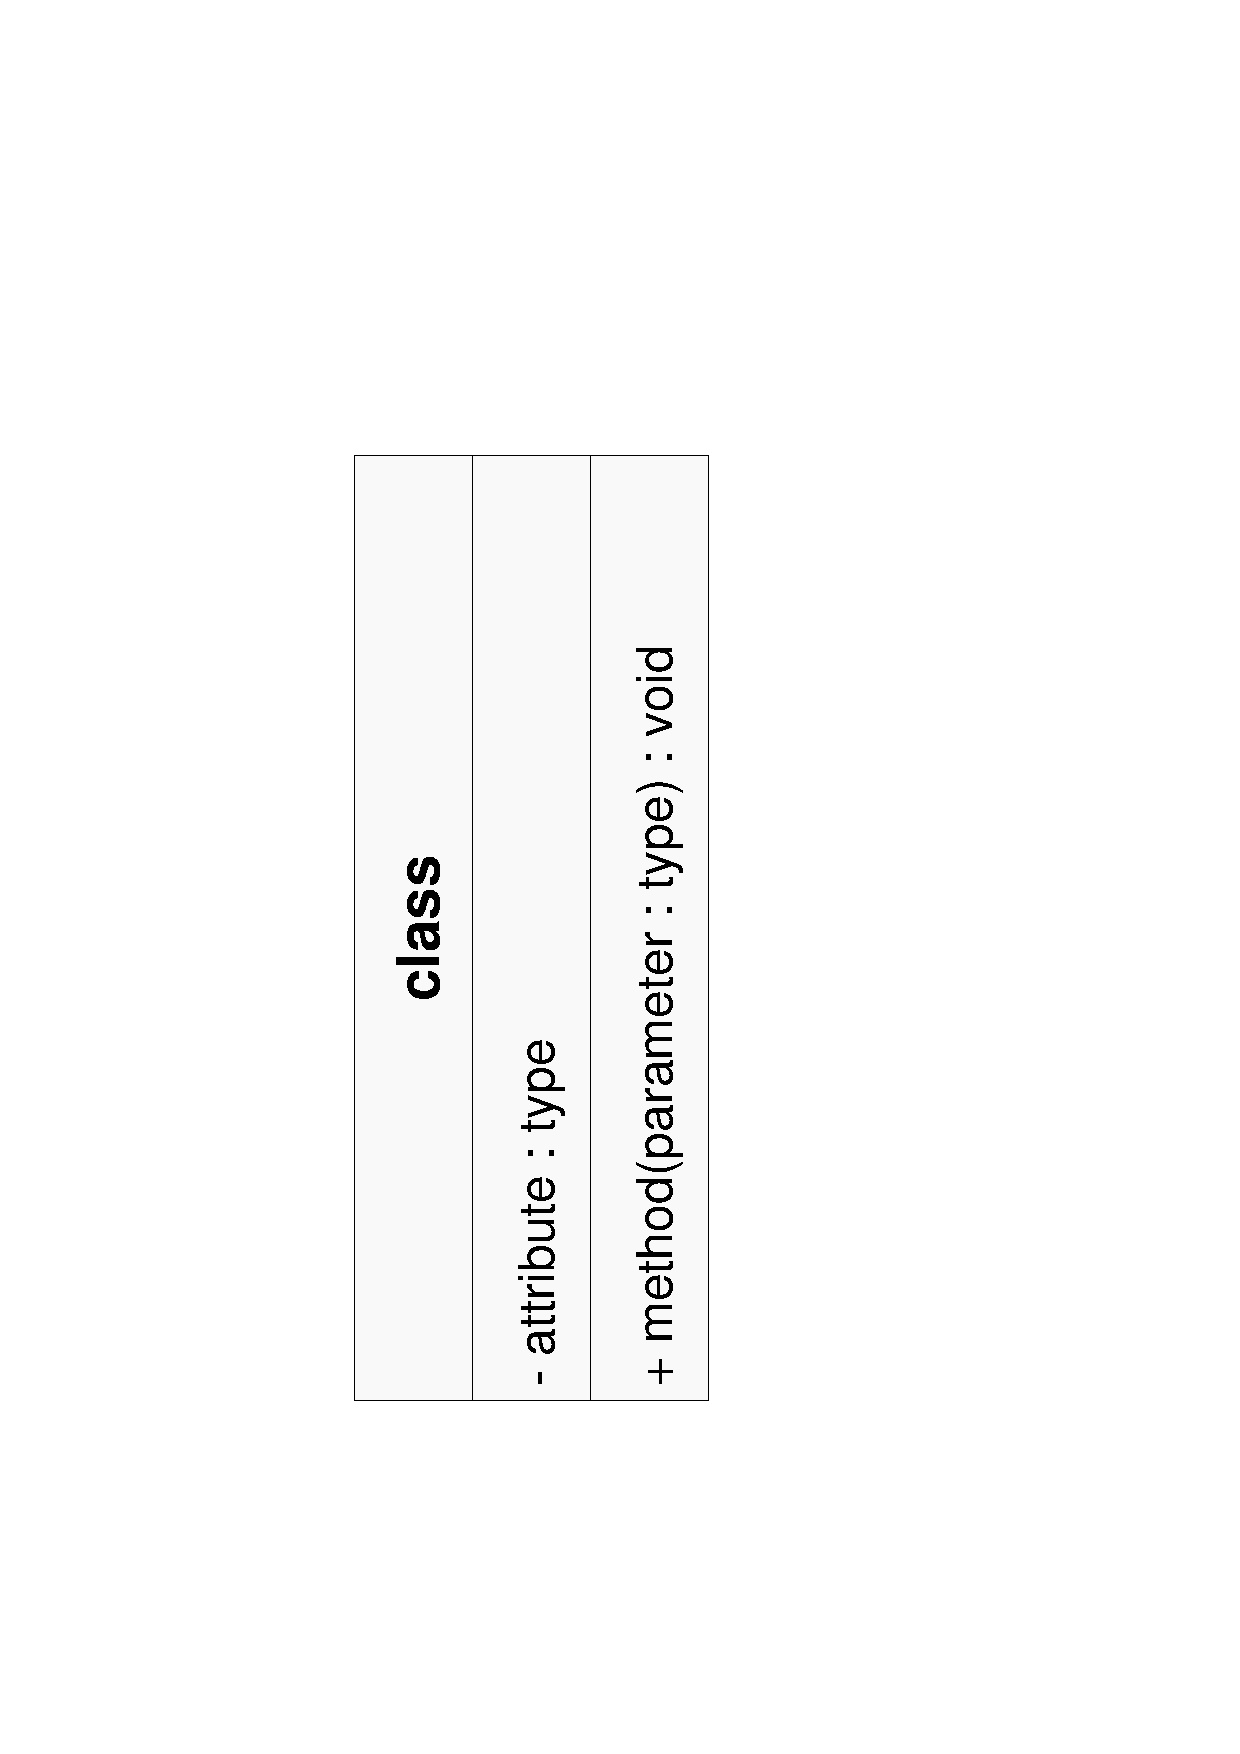
\includegraphics[scale=0.3,angle=-90]{graphic/classification.pdf}
        \caption{Classification as UML Diagram}
        \label{classification_figure}
    \end{center}
\end{figure}

While procedures and many variables in SPP are global, that is only exist once,
classes are treated as types of which many \emph{Instances} (also called
\emph{Objects}) can be created, including attributes and methods. In OOP, such
memory allocation is called \emph{Instantiation}.

Two related data types are \emph{Abstract Class} and \emph{Interface}. An
abstract class can hold attributes and (partly abstract) methods. Just like
interfaces, abstract classes cannot be instantiated. An interface is yet more
restricted in that it can only have constants but not attributes and only
declarations but not actual implementations of methods. Interfaces are commonly
used to \cite{steppan}:

\begin{itemize}
    \item[-] Realise multiple inheritance (section \ref{inheritance_heading})
    \item[-] Encapsulate components (section \ref{interface_and_implementation_heading})
    \item[-] Pool common methods (section \ref{separation_of_concerns_heading})
\end{itemize}

Specialities like \emph{Inner Classes} \cite{java} with limited scope of
validity are of minor importance to the argumentation of this document and not
further explained here.

The \emph{Bundling} of attributes and methods (state and logic) causes more
system interdependencies and complications than were predictable. It is a big
disadvantage that affects all modern object-oriented systems. \cite{heller2004}
Certainly, the bundling stems from best intentions to receive cleaner code by
keeping not only attributes but also methods in a common module, such avoiding
\emph{wild} and \emph{global} procedures. But now, modules not only have to
refer to other modules for accessing their state data; the same is needed for
accessing their logic in form of method calls.

With OOP, the number of cross-relations between modules, and inter-dependencies
between system layers may rise dramatically. In reality, state- and logic
properties are two \emph{different} things that have to be kept in different
places! Both can have a similar, hierarchical structure but each is a concept on
its own, as chapter \ref{state_and_logic_heading} will show.

%
% $RCSfile: examples.tex,v $
%
% Copyright (c) 2004. Christian Heller. All rights reserved.
%
% No copying, altering, distribution or any other actions concerning this
% document, except after explicit permission by the author!
% At some later point in time, this document is planned to be put under
% the GNU FDL license. For now, _everything_ is _restricted_ by the author.
%
% http://www.cybop.net
% - Cybernetics Oriented Programming -
%
% http://www.resmedicinae.org
% - Information in Medicine -
%
% @author Christian Heller <christian.heller@tuxtax.de>
%

\subsection{Examples}
\label{examples_heading}

This section briefly describes a greater number of known patterns. They are
basic examples referenced by the pattern systematics introduced in section
\ref{categories_heading}, later-on. However, since this section does not want to
copy the work accomplished by the aforementioned authors, it refers to the
corresponding literaric source for more detailed explanation.

%
% $RCSfile: architectural.tex,v $
%
% Copyright (c) 2004. Christian Heller. All rights reserved.
%
% No copying, altering, distribution or any other actions concerning this
% document, except after explicit permission by the author!
% At some later point in time, this document is planned to be put under
% the GNU FDL license. For now, _everything_ is _restricted_ by the author.
%
% http://www.cybop.net
% - Cybernetics Oriented Programming -
%
% http://www.resmedicinae.org
% - Information in Medicine -
%
% @author Christian Heller <christian.heller@tuxtax.de>
%

\subsubsection{Architectural}
\label{architectural_heading}

\emph{Architectural Patterns} are templates for the gross design of software
systems. They describe concrete software architectures and provide basic
structuring (modularization) principles.

\input{layers}
\input{data_mapper}
\input{data_transfer_object}
\input{model_view_controller}
\input{hierarchical_model_view_controller}
\input{microkernel}
\input{broker}
\input{pipes_and_filters}
\input{reflection}

%
% $RCSfile: design.tex,v $
%
% Copyright (C) 2002-2008. Christian Heller.
%
% Permission is granted to copy, distribute and/or modify this document
% under the terms of the GNU Free Documentation License, Version 1.1 or
% any later version published by the Free Software Foundation; with no
% Invariant Sections, with no Front-Cover Texts and with no Back-Cover
% Texts. A copy of the license is included in the section entitled
% "GNU Free Documentation License".
%
% http://www.cybop.net
% - Cybernetics Oriented Programming -
%
% http://www.resmedicinae.org
% - Information in Medicine -
%
% Version: $Revision: 1.1 $ $Date: 2008-08-19 20:41:06 $ $Author: christian $
% Authors: Christian Heller <christian.heller@tuxtax.de>
%

\subsection{Design}
\label{design_heading}
\index{Design Pattern}

Gamma et al. \cite{gamma1995} define a design pattern as: \textit{description of
collaborating objects and classes which are taylored to solve a general design
problem in a special context.} Mostly, patterns are in relation to each other.
They can be combined to master more complex tasks.

\input{command}
\input{wrapper}
\input{whole_part}
\input{composite}
\input{chain_of_responsibility}
\input{observer}
\input{bidirectional_dependency}

%
% $RCSfile: idiomatic.tex,v $
%
% Copyright (C) 2002-2008. Christian Heller.
%
% Permission is granted to copy, distribute and/or modify this document
% under the terms of the GNU Free Documentation License, Version 1.1 or
% any later version published by the Free Software Foundation; with no
% Invariant Sections, with no Front-Cover Texts and with no Back-Cover
% Texts. A copy of the license is included in the section entitled
% "GNU Free Documentation License".
%
% http://www.cybop.net
% - Cybernetics Oriented Programming -
%
% http://www.resmedicinae.org
% - Information in Medicine -
%
% Version: $Revision: 1.1 $ $Date: 2008-08-19 20:41:07 $ $Author: christian $
% Authors: Christian Heller <christian.heller@tuxtax.de>
%

\subsection{Idiomatic}
\label{idiomatic_heading}
\index{Idiomatic Pattern}
\index{Idiom}
\index{Counted Pointer Pattern}
\index{Singleton Pattern}
\index{Template Method Pattern}
\index{Factory Method Pattern}
\index{Envelope Letter Pattern}

An \emph{Idiom} is a pattern on a low abstraction level. It describes how certain
aspects of components or the relations between them can be implemented using the
means of a specific programming language. Idioms can thus be used to describe
the actual realisation of design patterns. Besides the \emph{Counted-Pointer}
pattern, Buschmann \cite[p. 377]{buschmann} also categorises \emph{Singleton},
\emph{Template Method}, \emph{Factory Method} and \emph{Envelope-Letter}
\cite{coplien} as \emph{Idiom}.

\input{template_method}
\input{counted_pointer}
\input{singleton}
\input{global_access}



    %
% $RCSfile: problems.tex,v $
%
% Copyright (c) 2004. Christian Heller. All rights reserved.
%
% No copying, altering, distribution or any other actions concerning this
% document, except after explicit permission by the author!
% At some later point in time, this document is planned to be put under
% the GNU FDL license. For now, _everything_ is _restricted_ by the author.
%
% http://www.cybop.net
% - Cybernetics Oriented Programming -
%
% http://www.resmedicinae.org
% - Information in Medicine -
%
% @author Christian Heller <christian.heller@tuxtax.de>
%

\section{Problems}
\label{problems_heading}

This section does not describe further patterns. Instead, it wants to come back
to reflective- and other mechanisms as described in section \ref{pattern_heading}
before, and elaborate their negative effects a bit more. Although the first of
the following three reviews concentrates on the example of \emph{Java}, many
points surely count for other \emph{Object Oriented Programming} (OOP) languages
as well.

%
% $RCSfile: broken_type_system.tex,v $
%
% Copyright (c) 2004. Christian Heller. All rights reserved.
%
% No copying, altering, distribution or any other actions concerning this
% document, except after explicit permission by the author!
% At some later point in time, this document is planned to be put under
% the GNU FDL license. For now, _everything_ is _restricted_ by the author.
%
% http://www.cybop.net
% - Cybernetics Oriented Programming -
%
% http://www.resmedicinae.org
% - Information in Medicine -
%
% @author Christian Heller <christian.heller@tuxtax.de>
%

\subsection{Broken Type System}
\label{broken_type_system_heading}

Languages like \emph{Smalltalk} or the \emph{Common Lisp Object System} (CLOS)
offer reflective mechanisms \cite{buschmann}. The \emph{C++ Standard Library},
also known as \emph{libstdc++} \cite{libstdcpp}, has a \emph{type\_info} class
providing meta information that \emph{C++} innately does not have.

In the \emph{Java} framework \cite{java}, finally, the basic \emph{java.lang.*}
package contains the top-most super class \emph{java.lang.Object}. All other
classes in the framework inherit from it. Additionally, the package contains a
class \emph{java.lang.Class} which, among others, keeps reflective (meta) type
information about a \emph{Java} class':

\begin{itemize}
    \item[-] Package
    \item[-] Name
    \item[-] Superior Class
    \item[-] Interfaces
    \item[-] Fields
    \item[-] Methods
    \item[-] Constructors
    \item[-] Modifiers
    \item[-] Member Classes
\end{itemize}

\begin{figure}[ht]
    \begin{center}
        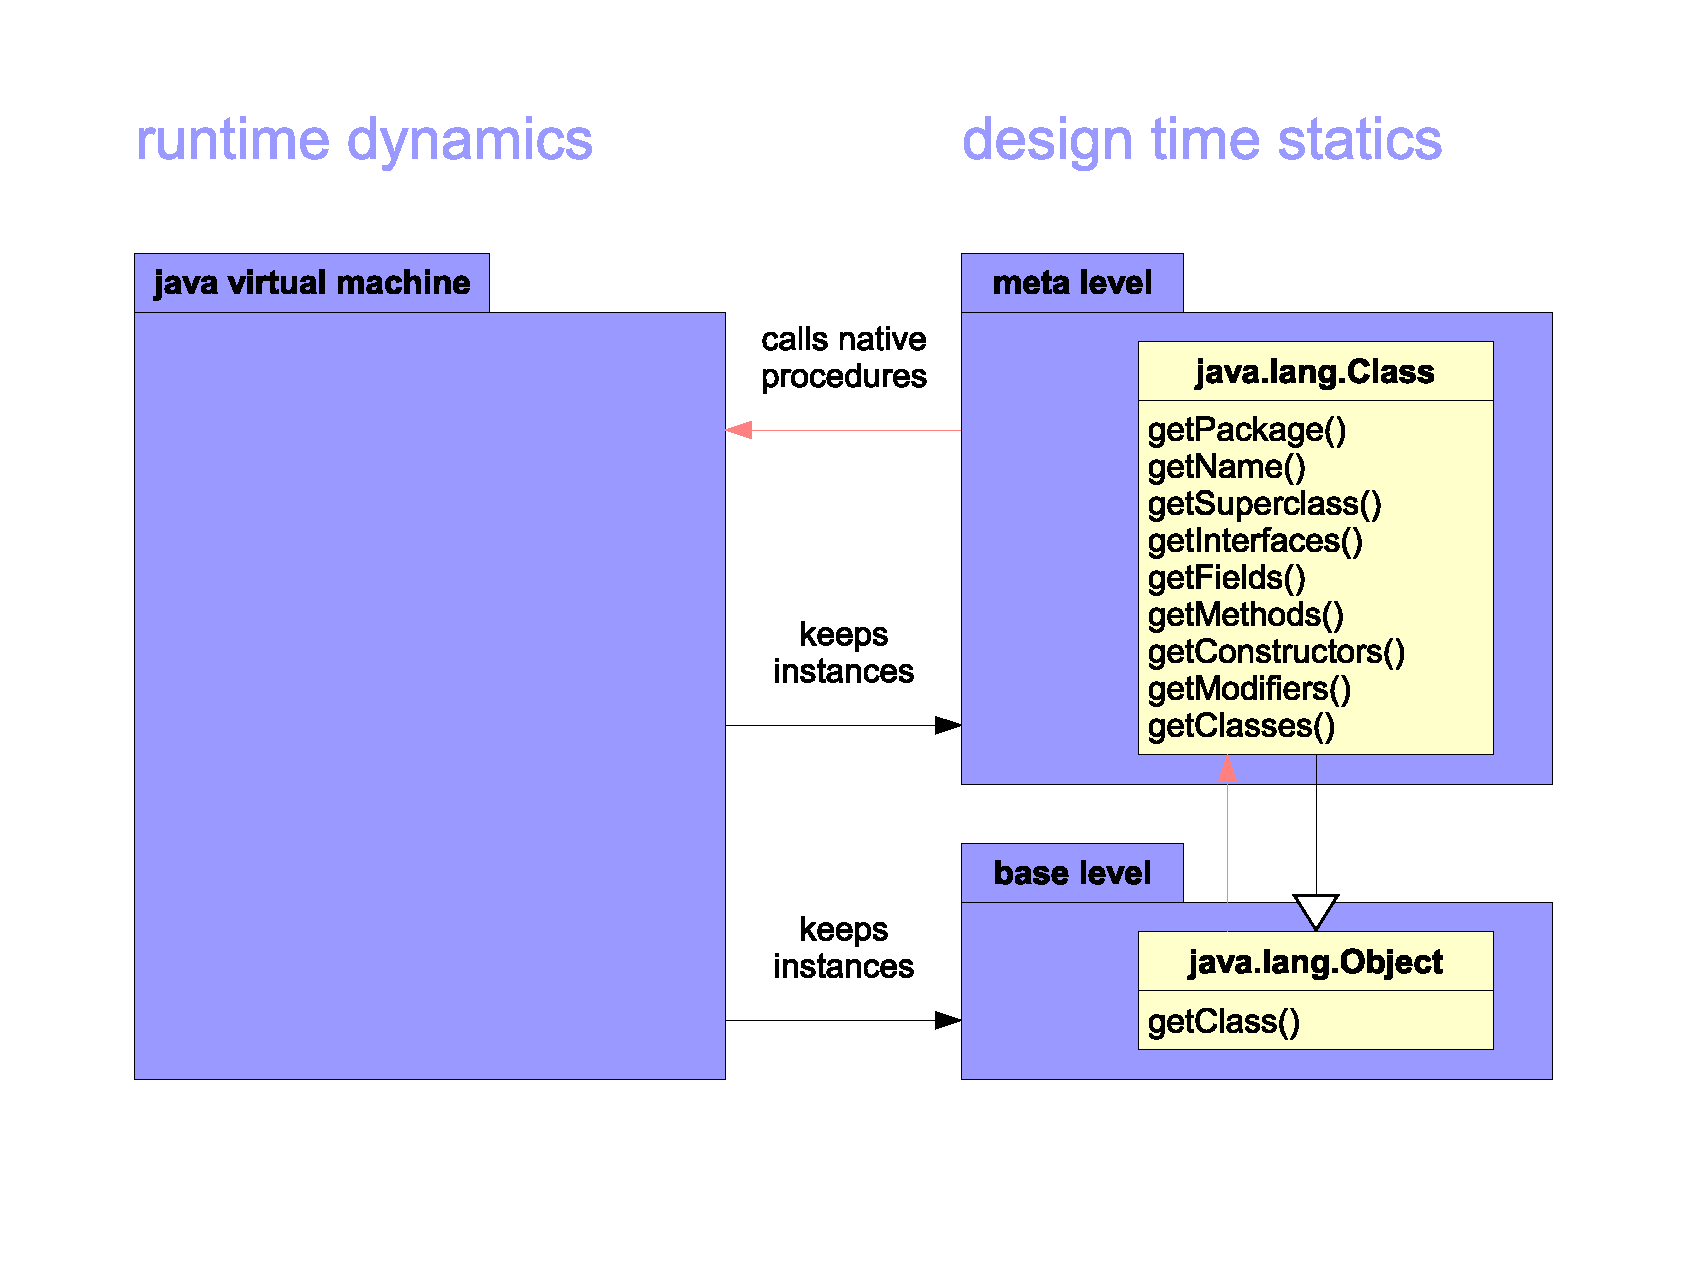
\includegraphics[scale=0.3]{vector/typesystem.eps}
        \caption{Java Type System}
        \label{typesystem_figure}
    \end{center}
\end{figure}

Via the \emph{getClass()} method which they inherit from \emph{java. lang.Object}
(figure \ref{typesystem_figure}), all Java classes have access to that reflective
information in their meta class. The meta class \emph{java.lang.Class} itself
uses so-called \emph{native} methods to access the information in the
\emph{Java Virtual Machine} (JVM).

The JVM operates on a level underneath the actual application, close to the
\emph{Operating System} (OS). It interprets the Java application source code and
resolves all object-oriented- into procedural structures, and finally low-level
system instructions. All runtime objects, that is class instances, are hold in
dynamic structures internal to the JVM. That is why \emph{native} methods need
to be used to access and change the runtime structure or behaviour of objects.

One problem that becomes obvious when inspecting figure \ref{typesystem_figure}
is the existence of a \emph{Bidirectional Dependency}, also called
\emph{Circular Reference}. The two sub dependencies causing it are:

\begin{enumerate}
    \item \emph{Inheritance} of \emph{java.lang.Class} from \emph{java.lang.Object}
        which is due to the rule that all Java classes need to inherit from the
        top-most framework class
    \item \emph{Association} from \emph{java.lang.Object} to \emph{java.lang.Class}
        which enables every object to access its meta class using the
        \emph{getClass()} method
\end{enumerate}

The avoidance of circular references is one of the most basic principles of
computer programming (section \ref{bidirectional_dependency_heading}). The
disadvantage of bidirectional dependencies between meta- and basic level is
also mentioned by Buschmann \cite{buschmann}. If meta classes in the kind of
\emph{java.lang.Class} define the structure and behaviour of all basic classes
inheriting from \emph{java.lang. Object}, then those meta classes in turn should
\emph{not} themselves inherit from \emph{java.lang.Object}.

Another problem is the mixed and redundant storage of meta information which
Jonathon Tidswell \cite{josgeneral} even calls a \emph{Broken Type System}. He
writes: \textit{A careful examination of the classes in the standard runtime will
show that they are not strictly instances of java.lang.Class (hint: statics).}
Gilbert Carl Herschberger II \cite{josgeneral} calls the separation of
reflection and wrappers an \emph{Inconsistent Design}. Java classes are based
on many different kinds of type information:

\begin{itemize}
    \item[-] Structure applied by the JVM through the usage of the \emph{class} keyword
    \item[-] Meta information supplied by the \emph{java.lang.Class} class
    \item[-] Reflective information provided by \emph{java.lang.reflect.*}
    \item[-] Wrapper classes for primitive types in \emph{java.lang.*}
    \item[-] Dynamically created array classes, without having an array class file
\end{itemize}

The fact that the \emph{java.lang.Class} class which is to provide meta
information \emph{about} classes is a \emph{Class} itself is an antagonism. It
is true that that meta class is made \emph{final} to avoid its extension by
inheriting subclasses. But correctly, it should not be a class at all.

Yet how can this paradoxon be resolved? Obviously, one of the two dependencies
between \emph{java.lang.Object} and \emph{java.lang.Class} needs to be cut. But
then either the \emph{java.lang. Object} class would not be able to access its meta
information anymore or the \emph{java.lang.Class} class would not be available as
runtime object to other polymorphic data structures. One solution could be to
merge both classes, so that each object, by default, has the necessary methods
to access its meta information. But as it turns out, this would not be a real
solution, just a \emph{Shift} of the problem to another level. As mentioned above,
the JVM keeps all instances (objects) in internal, dynamic structures. If objects
were allowed to access these internal structures via native methods (procedures),
a similar kind of bidirectional dependency, between the JVM and its stored objects,
would occur.

One finally has to ask whether the usage and manipulation of meta information is
really necessary at all! If objects did not have a \emph{static} structure
consisting of certain attributes and methods, as defined by the software
developer at design time, but instead based on a uniform, \emph{dynamically}
changeable structure -- the need to use reflective mechanisms might disappear.
More research has to be done on this topic.

There are other Java-related points to be criticised. Although it is worth
noting they exist, these are \emph{not} explained in detail here, since this
document wants to focus on general concepts. Gilbert Carl Herschberger II
\cite{josgeneral} mentions the problematic issue of \emph{Pre-Conditions},
leading to corresponding \emph{Assumptions}. After him, such work-arounds were
necessary to break circular references in Java:

\begin{itemize}
    \item[-] Each JVM must pre-define an \emph{Internal Meta Class}, implemented
        in machine code and \emph{not} available as Java bytecode in a class file.
        The \emph{java.lang.Class} as base meta class for all Java classes depends
        on that internal meta class and assumes its existance.
    \item[-] A JVM pre-defines one \emph{Primordial Class Loader}, implemented in
        machine code and resolved at compile-time. Since additional class loaders
        need to know their meta class when being created, they have to assume the
        primordial class loader exists so that, using it, their meta class can be
        created first.
\end{itemize}

Jonathon Tidswell \cite{josgeneral} is of the opinion that there are a number of
security issues related to the design of Java, for example:

\begin{itemize}
    \item[-] Global names not local references are used for security
    \item[-] Wrappers and names are used for reflection
\end{itemize}

Even though most of the issues raised in this section are rather Java-specific,
many of them apply to other programming languages as well. \emph{Smalltalk}
\cite{smalltalk} and \emph{CLU} \cite{clu}, for example, make primitive types
look like classes and do not need special \emph{Wrapper} classes like Java. But
when digging deep enough, one will find that this is \emph{Syntactic Sugar}, as
Peter J. Landin used to call additions to the syntax of a computer language
that do not affect its expressiveness but make it \emph{sweeter} for humans to
use \cite{wikipedia}.

%
% $RCSfile: bidirectional_dependency.tex,v $
%
% Copyright (C) 2002-2008. Christian Heller.
%
% Permission is granted to copy, distribute and/or modify this document
% under the terms of the GNU Free Documentation License, Version 1.1 or
% any later version published by the Free Software Foundation; with no
% Invariant Sections, with no Front-Cover Texts and with no Back-Cover
% Texts. A copy of the license is included in the section entitled
% "GNU Free Documentation License".
%
% http://www.cybop.net
% - Cybernetics Oriented Programming -
%
% http://www.resmedicinae.org
% - Information in Medicine -
%
% Version: $Revision: 1.1 $ $Date: 2008-08-19 20:41:05 $ $Author: christian $
% Authors: Christian Heller <christian.heller@tuxtax.de>
%

\subsubsection{Bidirectional Dependency}
\label{bidirectional_dependency_heading}
\index{Bidirectional Dependency}
\index{Inter-Dependency}
\index{Endless Loop}
\index{Tree}
\index{Directed Acyclic Graph}
\index{DAG}
\index{Oriented Acyclic Graph}
\index{Process Tree}
\index{Object Tree}
\index{Database Data Structure}
\index{File System Structure}
\index{Syntax Tree}
\index{Acyclic Graph}
\index{Circular Reference}

\emph{Bidirectional References} are a nightmare for every software developer.
They cause \emph{Inter-Dependencies} so that changes in one part of a system can
affect multiple other parts which in turn affect the originating part, which may
finally lead to cycles or even endless loops. Also, the actual program flow and
effects of changes to a system become very hard to trace. Therefore, the avoidance
of such dependencies belongs to the core principles of good software design.

A \emph{Tree}, in mathematics, is defined as \textit{Directed Acyclic Graph}
(DAG), also known as \emph{Oriented Acyclic Graph} \cite{nist}. It has a
\emph{Root Node} and \emph{Child Nodes} which can become \emph{Parent Nodes}
when having children themselves; otherwise they are called \emph{Leaves}.
Children of the same node are \emph{Siblings}. \textit{A common constraint is
that no node can have more than one parent}, as \cite{foldoc} writes and
continues: \textit{Moreover, for some applications, it is necessary to consider
a node's children to be an ordered list, instead of merely a set.} A graph is
\emph{acyclic} if every node can be reached via exactly one path, which then
also is the shortest possible.

In computing, trees are used in many forms, for example as \emph{Process Tree}
of an operating system \cite{debian, gnu, linux} or as \emph{Object Tree} of an
object-oriented application. They represent \emph{Data Structures} in databases
or file systems and also the \emph{Syntax Tree} of languages. The violation of
the principle of the \emph{Acyclic Graph} can lead to the same loops, also
called \emph{Circular References}, as mentioned above, which can result in the
crossing of memory limits and is a potential security risk. Therefore, one of
the main aims in the creation of the new concepts introduced in part
\ref{contribution_heading} of this work was the avoidance of bidirectional
relations.

%
% $RCSfile: global_access.tex,v $
%
% Copyright (c) 2004. Christian Heller. All rights reserved.
%
% No copying, altering, distribution or any other actions concerning this
% document, except after explicit permission by the author!
% At some later point in time, this document is planned to be put under
% the GNU FDL license. For now, _everything_ is _restricted_ by the author.
%
% http://www.cybop.net
% - Cybernetics Oriented Programming -
%
% http://www.resmedicinae.org
% - Information in Medicine -
%
% @author Christian Heller <christian.heller@tuxtax.de>
%

\subsection{Global Access}
\label{global_access_heading}

A pure tree of instances in a computer's \emph{Random Access Memory} (RAM)
represents an unidirectional structure that permits data access along
\emph{well-defined} paths. Global access via static types, on the other hand,
allows \emph{any} instance to address data in memory \emph{directly}, which not
only complicates software development and maintenance, but, due to the
uncontrollable access, is a potential security risk.

The usage of static objects accessible by any other part in a system is an
\emph{Anti Pattern} to \emph{Inversion of Control} (IoC) \cite{avalon}, highly
insecure and hence undesirable.


    %
% $RCSfile: new_systematics.tex,v $
%
% Copyright (c) 2004. Christian Heller. All rights reserved.
%
% No copying, altering, distribution or any other actions concerning this
% document, except after explicit permission by the author!
% At some later point in time, this document is planned to be put under
% the GNU FDL license. For now, _everything_ is _restricted_ by the author.
%
% http://www.cybop.net
% - Cybernetics Oriented Programming -
%
% http://www.resmedicinae.org
% - Information in Medicine -
%
% @author Christian Heller <christian.heller@tuxtax.de>
%

\section{New Systematics}
\label{new_systematics_heading}

Section \ref{pattern_heading} used traditional proposals \cite{buschmann,gamma1995}
to systematize patterns and divided them according to the first categorization
level shown in figure \ref{pattern_figure}. The following sections will work out
a new systematics, to classify patterns.

%
% $RCSfile: human_thinking.tex,v $
%
% Copyright (c) 2004. Christian Heller. All rights reserved.
%
% No copying, altering, distribution or any other actions concerning this
% document, except after explicit permission by the author!
% At some later point in time, this document is planned to be put under
% the GNU FDL license. For now, _everything_ is _restricted_ by the author.
%
% http://www.cybop.net
% - Cybernetics Oriented Programming -
%
% http://www.resmedicinae.org
% - Information in Medicine -
%
% @author Christian Heller <christian.heller@tuxtax.de>
%

\subsection{Human Thinking}
\label{human_thinking_heading}

The new classification is based on the idea of categorizing software patterns
after the principles of \emph{Human Thinking}, that is concepts of the logical
\emph{Mind}, as opposed to \emph{Artificial Neural Networks} (ANN) that want to
imitate the functioning of the physical \emph{Brain}.

The corresponding concepts were first introduced in \cite{heller2004}. After an
investigation of the fundamentals of human thinking, that is how human beings
understand their surrounding real world by abstracting it in \emph{Models}, that
paper concludes that there were three basic activities of abstraction:

\begin{enumerate}
    \item Discrimination
    \item Categorization
    \item Composition
\end{enumerate}

By discriminating their environment, humans are able to share it into discrete
\emph{Items}. Items with similar properties can be classified into a common super
\emph{Category}. Any abstract model of the universe is just an illusion, being
made up of yet smaller models, and nobody knows where this hierarchy really stops,
towards microcosm as well as towards macrocosm. Therefore, the third and last
kind of abstraction, namely composition, lets humans perceive the items in their
environment as \emph{Compound} of smaller items.

\begin{figure}[ht]
    \begin{center}
        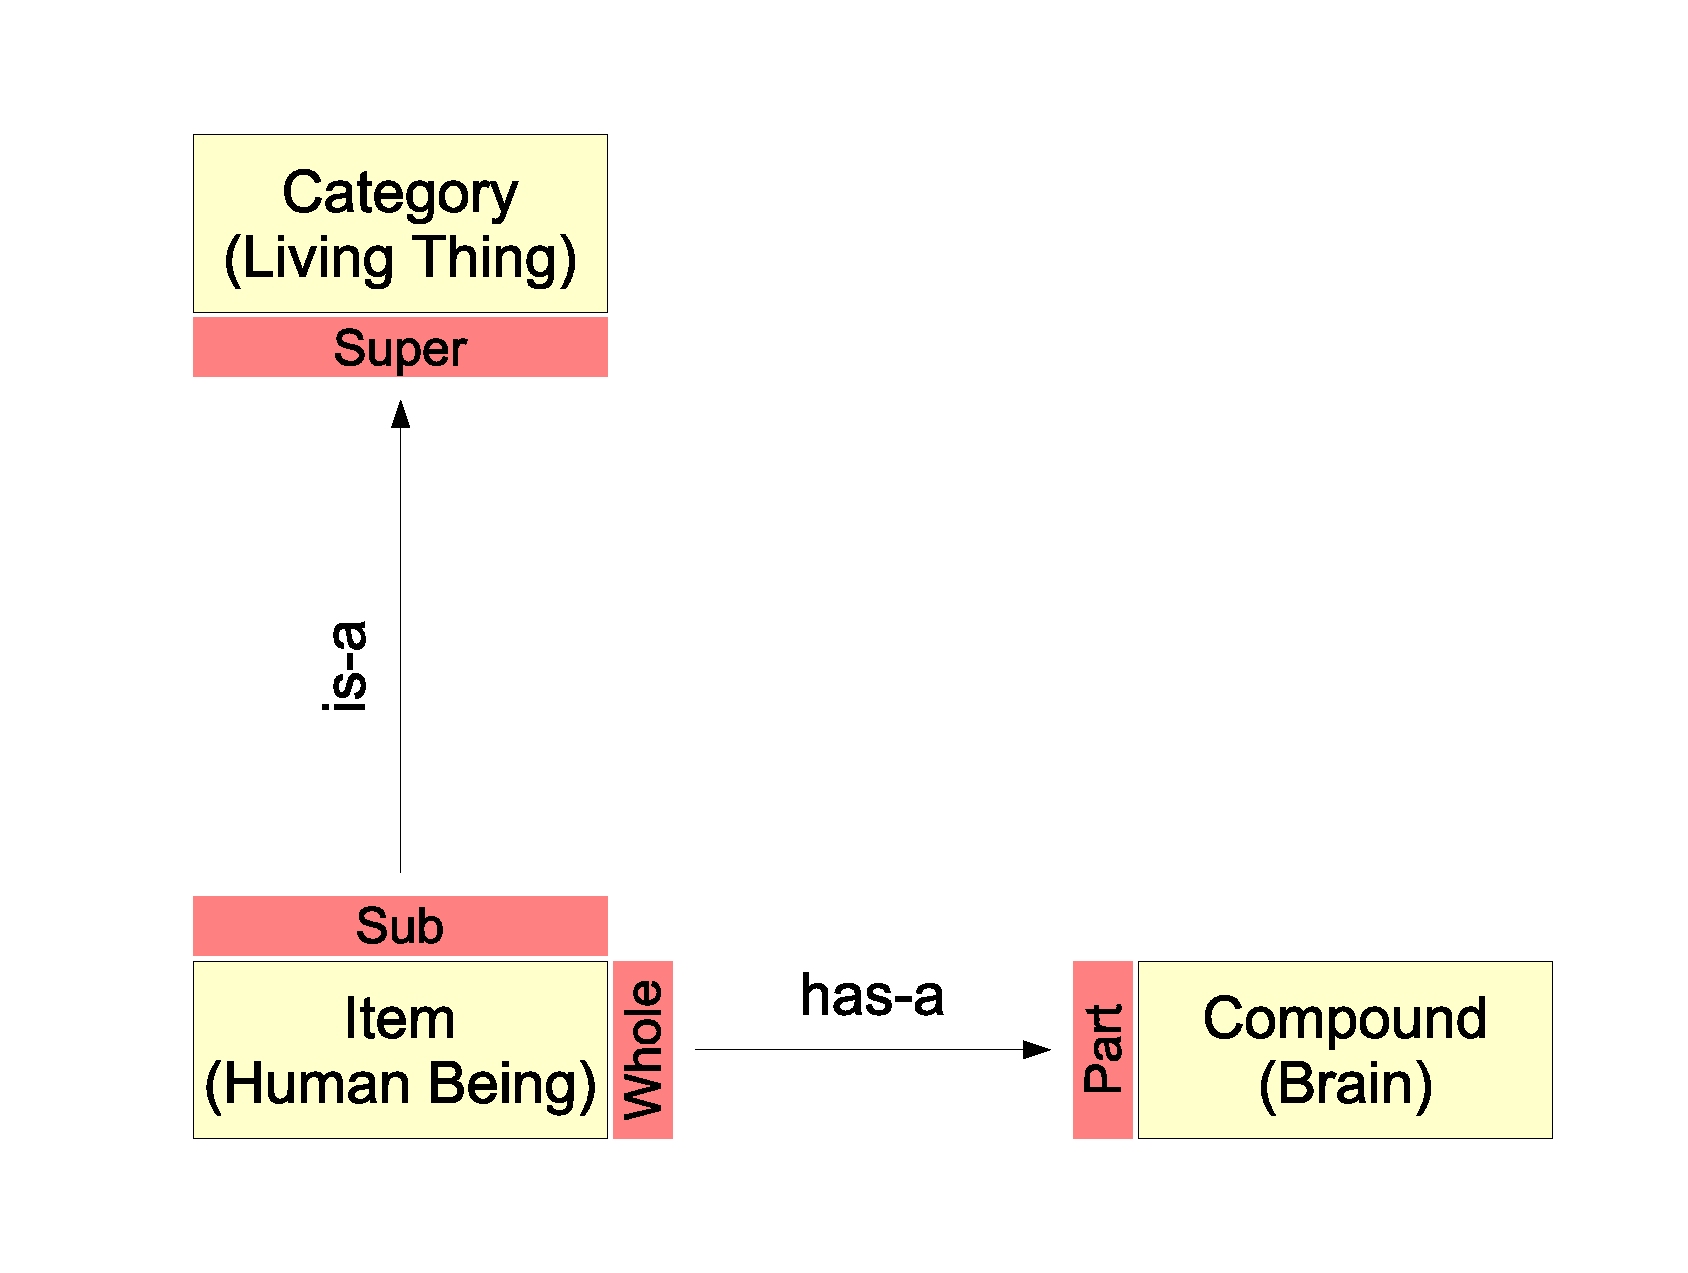
\includegraphics[scale=0.3]{vector/abstraction.eps}
        \caption{Abstractions of Human Thinking \cite{heller2004}}
        \label{abstraction_figure}
    \end{center}
\end{figure}

The latter two activities of abstraction -- categorization and composition --
are based on special \emph{Associations} (figure \ref{abstraction_figure}),
between a \emph{Super-} and a \emph{Sub} model and between a \emph{Whole-} and
a \emph{Part} model, respectively.

%
% $RCSfile: categories.tex,v $
%
% Copyright (c) 2004. Christian Heller. All rights reserved.
%
% No copying, altering, distribution or any other actions concerning this
% document, except after explicit permission by the author!
% At some later point in time, this document is planned to be put under
% the GNU FDL license. For now, _everything_ is _restricted_ by the author.
%
% http://www.cybop.net
% - Cybernetics Oriented Programming -
%
% http://www.resmedicinae.org
% - Information in Medicine -
%
% @author Christian Heller <christian.heller@tuxtax.de>
%

\subsection{Categories}
\label{categories_heading}

Most patterns heavily rely on associations, too. This paper therefore suggests to:

\begin{center}
    \textbf{Take the Kind of Association as Criterion\\
    to sort patterns in a completely new way.}
\end{center}

The opposite table shows a systematics of the new pattern categories with their
equivalents in human thinking, some representative example patterns and a
recommendation for their usage in software engineering. Patterns matching into
more than one category are placed after the priority: \emph{Recursion} over
\emph{Polymorphism}.

\begin{table}[ht]
    \begin{center}
        \begin{tabular}{| p{22mm} | p{20mm} | p{23mm} | p{10mm} |}
            \hline
            \textbf{Category} & \textbf{Equivalent} & \textbf{Representative} & \textbf{Advice}\\
            \hline
            Itemization & Discrimination & Command, Data Transfer Object, State, Memento, Envelope-Letter, Prototype & :-)\\
            \hline
            1:1 Association & Composition & Delegator, Object Adapter, Proxy (Surrogat, Client-/Server Stub), Wrapper, Handle-Body, Bridge & :-)\\
            \hline
            1:n Association & Composition & Whole-Part, View Handler, Broker (Mediator), Master-Slave, Command Processor, Counted Pointer, Chain of Responsibility & :-)\\
            \hline
            Recursion & Composition & Composite, Interpreter, Decorator, Linked Wrapper & :-)\\
            \hline
            Bidirectionalism & -- & Observer (Callback, Publisher-Subscriber), Forwarder-Receiver, Chain of Responsibility, Visitor, Reflection & :-(\\
            \hline
            Polymorphism & Categorization & Template Method, Builder, Factory Method, Class Adapter, Abstract Factory (Kit), Strategy (Validator, Policy), Iterator (Cursor) & :-$\mid$\\
            \hline
            Grouping & Categorization & Layers, Domain Model, MVC & :-)\\
            \hline
            Global Access & -- & Singleton, Flyweight, Registry, Manager & :-(\\
            \hline
        \end{tabular}
%        \caption{Pattern Systematics}
        \label{pattern_systematics_table}
    \end{center}
\end{table}

%
% $RCSfile: recommendation.tex,v $
%
% Copyright (c) 2004. Christian Heller. All rights reserved.
%
% No copying, altering, distribution or any other actions concerning this
% document, except after explicit permission by the author!
% At some later point in time, this document is planned to be put under
% the GNU FDL license. For now, _everything_ is _restricted_ by the author.
%
% http://www.cybop.net
% - Cybernetics Oriented Programming -
%
% http://www.resmedicinae.org
% - Information in Medicine -
%
% @author Christian Heller <christian.heller@tuxtax.de>
%

\subsection{Recommendation}
\label{recommendation_heading}

The first category \emph{Itemization} (objectification) is the base of any
modelling activity and clearly necessary.

The next three categories \emph{1:1 Association}, \emph{1:n Association} and
\emph{Recursion} are special kinds of associations that rely exclusively on
\emph{unidirectional} relations and result in a clean architecture which is why
their usage is strongly recommended.

\emph{Bidirectionalism}, on the other hand, is an \emph{ill} variant of the three
aforementioned categories and should be avoided wherever possible. Patterns in
this category are one reason for endless loops and unpredictable behaviour since
it becomes very difficult to trace the effects that changes in one place of a
system have on others (section \ref{bidirectional_dependency_heading}).

\emph{Polymorphism} is a good thing. It relies on categorization and due to
inheritance can avoid a tremendous amount of otherwise redundant source code.
However, it also makes understanding a system more difficult, since the whole
architecture must be understood before being able to manipulate code correctly.
Unwanted source code changes caused by inheritance dependencies are often
described with the term \emph{Fragile Base Class Problem}
\cite[section \emph{Layers}]{buschmann}. They are just the opposite of what
inheritance was actually intended to be for: \emph{Reusability}
\cite[Vorwort]{gruhn}.

\emph{Grouping} models is essential to keep overview in a complex software
system. A very promising technology to support this are \emph{Ontologies}
\cite{hellerkunze}. A lot of thought-work has to go into them but if they are
well thought-out, they are clearly recommended.

The habit of globally accessing models is banned since OOP became popular.
However, it is not banned completely. Patterns like \emph{Singleton}
encapsulate and bundle global access but they still permit it. They disregard
any dependencies and relations in a system, such are a security risk and reason
for untraceable data changes. This paper sees the whole category of
\emph{Global Access} as potentially dangerous and can \emph{not} recommend its
patterns.


    %
% $RCSfile: summary.tex,v $
%
% Copyright (c) 2001-2004. Christian Heller. All rights reserved.
%
% No copying, altering, distribution or any other actions concerning this
% document, except after explicit permission by the author!
% At some later point in time, this document is planned to be put under
% the GNU FDL license. For now, _everything_ is _restricted_ by the author.
%
% http://www.cybop.net
% - Cybernetics Oriented Programming -
%
% http://www.resmedicinae.org
% - Information in Medicine -
%
% @author Christian Heller <christian.heller@tuxtax.de>
%

\section{Summary}
\label{summary_heading}

This paper means that wild \emph{Dependencies} are a major reason for error-prone,
unstable, unflexible, unmaintainable software systems. Two facts causing such
dependencies are the \emph{Bundling} of static and dynamic properties by
object-oriented languages and the \emph{Mix} of knowledge and hardware control
in traditional programming languages. This information mix additionally forces
software development projects to run through a course of different abstraction
steps which would not differ if one common knowledge abstraction were used.

As solution to the above's problems, this document suggests to build software
systems after the concepts of \emph{Human Thinking}. The approach, named CYBOP,
such follows the recommendations of the science of \emph{Cybernetics} and its
specialization \emph{Bionics}, whereby biological principles should be applied
to the study and design of engineering systems. An abstract model as formed in the
human mind represents an \emph{Item}, \emph{Category} and \emph{Compound}, at the
same time. Additionally, it contains \emph{Meta Information} about its parts.
This information often corresponds to physical dimensions and determines whether
the model is an abstraction of \emph{static} or \emph{dynamic} real-world aspects.

The introduced \emph{CYBOL} language has the semantics to express knowledge models
as used by human thinking. It allows to create complete application systems. Its
syntax is based on \emph{XML} which results in absolutely platform- independent
system definitions. CYBOL files get interpreted by the \emph{CYBOI} interpreter
and can be changed at runtime. CYBOI manages all hardware access. It concentrates
model instances and signal handling in one place and such avoids memory leaks and
endless loops.

CYBOL models could be displayed graphically, using special design tools. But their
\emph{formal definition} also allows them to be used as main abstraction throughout
all phases in a software project's lifetime. Analysts and experts can start their
work by creating rudimentary CYBOL models (defining static structures and dynamic
processes) which software designers can later complete and check for correctness.
The implementation phase becomes superfluous at all: CYBOL models already represent
the system to be built, no further code is needed! It is hard to imagine the amount
of saved time and costs for software projects. Even better: Experts are placed in
a position to, themselves, actively help creating systems.

    \label{references_heading}
    \bibliographystyle{plain}
    \bibliography{references}
\end{document}
